\usetikzlibrary{arrows,shapes,positioning,shadows,trees}
\usetikzlibrary{decorations.pathmorphing} % Pour obtenir des lignes de coupes aléatoires
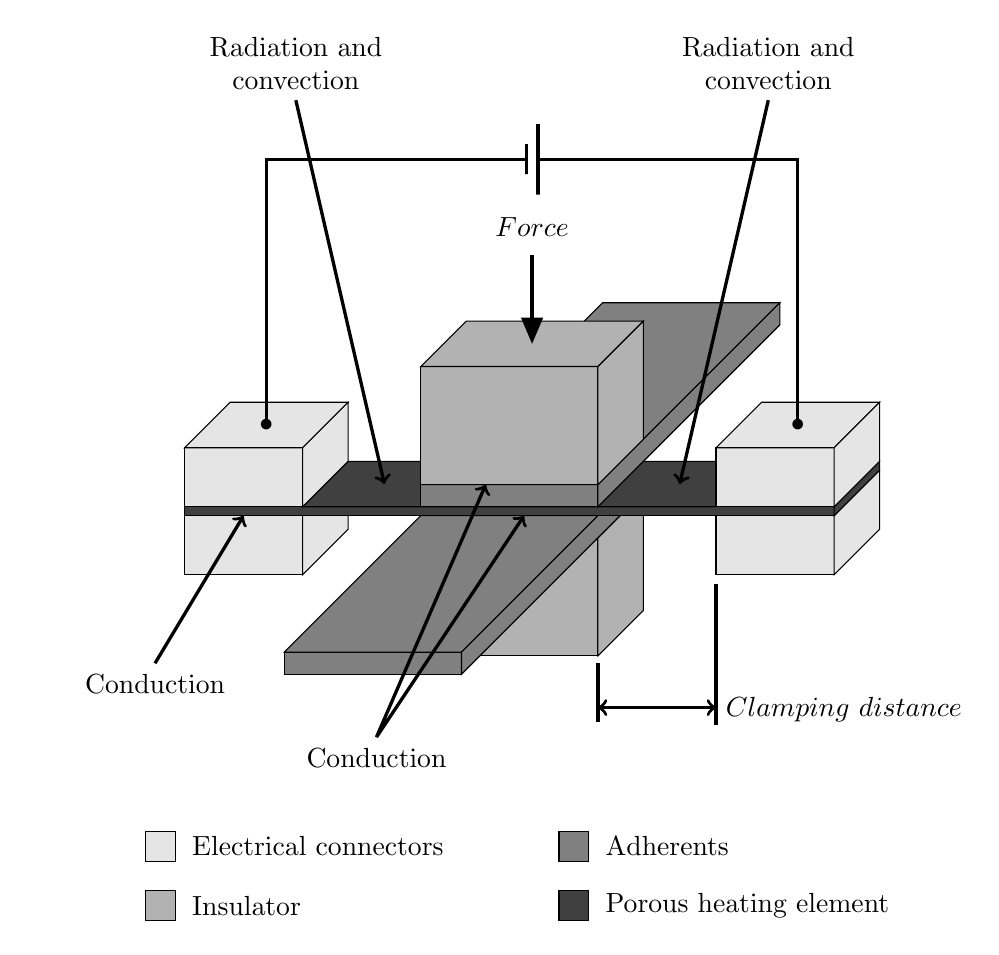
\begin{tikzpicture}[scale=0.75]


%Dimentions du bloc de connection
\def \largconnection{2}
\def \profconnection{2}
\def \hconnection{1.}

%Distance entre les deux blocs
\def \distance_connection{9}

%Épaisseur de l'élément résistif
\def \tele{0.15}

%Distance entre les blocs de connection et l'isolant
\def \gap{2}

%Dimensions des adhérent
\def \lcomp{6}
\def \tcomp{0.375}

%Épaisseur de l'isolant
\def \tbloc{2}

%Position et taille des annotations
\def \hsource{1.25*\profconnection}
\def \hpression{0.75*\profconnection}
\def \legende{0.5}
\def \distcotation{0.125}

%Couleurs
\def \colinsulator{blue!50}
\def \coladherend{green!50}
\def \colconnector{orange!60}
\def \colresistive{gray!50}

\def \colinsulator{black!30}
\def \coladherend{black!50}
\def \colconnector{black!10}
\def \colresistive{black!75}

%Bloc de pression inferieur
\draw[black,fill=\colinsulator] (\largconnection+\gap,-\tcomp-\tele-\tbloc,0) -- ++(0,\tbloc,0) -- ++(\distance_connection-\gap-\gap-\largconnection,0,0) -- ++(0,-\tbloc,0) -- cycle; %Face du devant
\draw[black,fill=\colinsulator] (\distance_connection-\gap,-\tcomp-\tele-\tbloc,0) -- ++(0,\tbloc,0) -- ++(0,0,-\profconnection) -- ++(0,-\tbloc,0) -- cycle; %Face de droite

%Adherant inferieur
\draw[black,fill=\coladherend] (\largconnection+\gap,-\tele-\tcomp,\lcomp) -- ++(0,\tcomp,0) -- ++(\distance_connection-\gap-\gap-\largconnection,0,0) -- ++(0,-\tcomp,0) -- cycle; %Face du devant
\draw[black,fill=\coladherend] (\largconnection+\gap,-\tele,\lcomp) -- ++(0,0,-\lcomp) -- ++(\distance_connection-\gap-\gap-\largconnection,0,0) -- ++(0,0,\lcomp) -- cycle; %Face du dessus
\draw[black,fill=\coladherend] (\distance_connection-\gap,-\tele,\lcomp) -- ++(0,-\tcomp,0) -- ++(0,0,-\lcomp-\profconnection) -- ++(0,\tcomp,0) -- cycle; %Face de droite

%Connection gauche inferieur
\draw[black, fill=\colconnector] (0,-\tele-\hconnection,0)--++(\largconnection,0,0)--++(0,\hconnection,0)--++(-\largconnection,0,0)--cycle; %Face du devant
\draw[black, fill=\colconnector] (\largconnection,-\tele-\hconnection,0)--++(0,\hconnection,0)-- ++(0,0,-\profconnection)--++(0,-\hconnection,0)--cycle; %Face de droite

%Connection droite inferieur
\draw[black, fill=\colconnector] (\distance_connection,-\tele-\hconnection,0)--++(\largconnection,0,0)--++(0,\hconnection,0)--++(-\largconnection,0,0)--cycle; %Face du devant
\draw[black, fill=\colconnector] (\largconnection+\distance_connection,-\tele-\hconnection,0)--++(0,\hconnection,0)--++(0,0,-\profconnection)--++(0,-\hconnection,0)--cycle; %Face de droite

%Element chauffant
\draw[black,fill=\colresistive] (0,0,0) -- (\largconnection+\distance_connection,0,0) -- ++(0,-\tele,0) -- (0,-\tele,0) -- cycle; %Face du devant
\draw[black,fill=\colresistive] (\largconnection,0,0) -- ++(0,0,-\profconnection) -- (\distance_connection,0,-\profconnection) -- (\distance_connection,0,0) -- cycle; %Face du dessus
\draw[black,fill=\colresistive] (\distance_connection+\largconnection,0,0) -- ++(0,0,-\profconnection) -- ++(0,-\tele,0) -- ++(0,0,\profconnection) -- cycle; %Face de droite

%Adherant superieur
\draw[black,fill=\coladherend] (\largconnection+\gap,0,0) -- ++(0,\tcomp,0) -- ++(\distance_connection-\gap-\gap-\largconnection,0,0) -- ++(0,-\tcomp,0) -- cycle; %Face du devant
\draw[black,fill=\coladherend] (\largconnection+\gap,\tcomp,0) -- ++(0,0,-\lcomp-\profconnection) -- ++(\distance_connection-\gap-\gap-\largconnection,0,0) -- ++(0,0,\lcomp+\profconnection) -- cycle; %Face du dessus
\draw[black,fill=\coladherend] (\distance_connection-\gap,\tcomp,0) -- ++(0,-\tcomp,0) -- ++(0,0,-\lcomp-\profconnection) -- ++(0,\tcomp,0) -- cycle; %Face de droite

%Connection gauche superieure
\draw[black, fill=\colconnector] (0,0,0)--(\largconnection,0,0)--++(0,\hconnection,0)--(0,\hconnection,0)--cycle; %Face du devant
\draw[black, fill=\colconnector] (0,\hconnection,0)--++(\largconnection,0,0)--++(0,0,-\profconnection)--++(-\largconnection,0,0)--cycle; %Face du dessus
\draw[black, fill=\colconnector] (\largconnection,0,0)--++(0,\hconnection,0)-- ++(0,0,-\profconnection)--++(0,-\hconnection,0)--cycle; %Face de droite

%Connection droite superieure
\draw[black, fill=\colconnector] (\distance_connection,0,0)--++(\largconnection,0,0)--++(0,\hconnection,0)--++(-\largconnection,0,0)--cycle; %Face du devant
\draw[black, fill=\colconnector] (\distance_connection,\hconnection,0)--++(\largconnection,0,0)--++(0,0,-\profconnection)--++(-\largconnection,0,-0)--cycle; %Face du dessus
\draw[black, fill=\colconnector] (\largconnection+\distance_connection,0,0)--++(0,\hconnection,0)--++(0,0,-\profconnection)--++(0,-\hconnection,0)--cycle; %Face de droite

%Bloc de pression superieur
\draw[black,fill=\colinsulator] (\largconnection+\gap,\tcomp,0) -- ++(0,\tbloc,0) -- ++(\distance_connection-\gap-\gap-\largconnection,0,0) -- ++(0,-\tbloc,0) -- cycle; %Face du devant
\draw[black,fill=\colinsulator] (\largconnection+\gap,\tcomp+\tbloc,0) -- ++(0,0,-\profconnection) -- ++(\distance_connection-\gap-\gap-\largconnection,0,0) -- ++(0,0,\profconnection) -- cycle; %Face du dessus
\draw[black,fill=\colinsulator] (\distance_connection-\gap,\tcomp,0) -- ++(0,\tbloc,0) -- ++(0,0,-\profconnection) -- ++(0,-\tbloc,0) -- cycle; %Face de droite

%Connection de la source de puissance
\draw [very thick] (0.5*\largconnection,\hconnection,-0.5*\profconnection) -- ++(0,\hsource+\tbloc,0) -- ++(0.5*\distance_connection-0.1,0,0) -- ++(0,-0.25,0) -- ++(0,0.5,0);
\draw [very thick] (0.5*\largconnection+\distance_connection,\hconnection,-0.5*\profconnection) -- ++(0,\hsource+\tbloc,0) -- ++ (-0.5*\distance_connection+0.1,0,0) -- ++(0,-0.6,0) -- ++ (0,1.2,0);
\draw (0.5*\largconnection,\hconnection,-0.5*\profconnection) node {$\bullet$} ;
\draw (0.5*\largconnection+\distance_connection,\hconnection,-0.5*\profconnection) node {$\bullet$} ;

%Pression
\draw [very thick, -triangle 45] (0.5*\largconnection+0.5*\distance_connection,\tbloc+\tcomp+\hpression,-0.5*\profconnection) -> ++(0,-\hpression,0);
\draw (0.5*\largconnection+0.5*\distance_connection,\tbloc+\tcomp+\hpression+0.15,-0.5*\profconnection) node[above] {$Force$};

%Clamping distance
\draw [very thick, black] (\distance_connection-\gap,-\tcomp-\tele-\tbloc-\distcotation,0) -- ++(0,-1,0);
\draw [very thick, black] (\distance_connection,-0.5*\tcomp-\hconnection-\distcotation,0) -- ++(0,-1-\tbloc+\hconnection-\tcomp,0);
\draw [very thick, black, <->] ((\distance_connection-\gap,-\tcomp-\tele-\tbloc-\distcotation-0.75,0) -- ++ (\gap,0,0);
\draw (\distance_connection,-0.5*\tcomp-\tcomp-\distcotation-\tbloc-.75,0) node[right] {$Clamping \ distance$};

%Identification des modes de refroidissement
\draw [very thick,<-] (\largconnection+0.5*\gap,0,-0.5*\profconnection) -- ++(-1.5,6.5,0) node[above, text width=3cm, align=center] {{Radiation and \\ convection}};
\draw [very thick,<-]  (\distance_connection-0.5*\gap,0,-0.5*\profconnection) -- ++(1.5,6.5,0) node[above, text width=3cm, align=center] {{Radiation and \\ convection}};
\draw [very thick,<-]  (0.5*\largconnection,-\tele,0) -- ++(-1.5,-2.5,0) node[below, text width=3cm, align=center] {{Conduction}};
\draw [very thick,<->]  (0.5*\distance_connection+0.625*\gap,-\tele,0) -- ++(-2.5,-3.75,0) node[below, text width=3cm, align=center] {{Conduction}} --(0.5*\distance_connection+0.3*\gap,\tcomp,0) ;


%Legende
\begin{scope}[yshift=-11.cm, xshift=-5.5cm]

	\begin{scope}[xshift=-7cm]
		\draw [black, fill=\colconnector] (\distance_connection+1.42*\profconnection,2.5*\tbloc) rectangle ++(\legende,\legende);
		\draw (\distance_connection+1.42*\profconnection+1.25*\legende,2.5*\tbloc+0.5*\legende) node[right]{Electrical connectors} ;

		\draw [black, fill=\colinsulator] (\distance_connection+1.42*\profconnection,2.5*\tbloc-2*\legende) rectangle ++(\legende,\legende);
		\draw (\distance_connection+1.42*\profconnection+1.25*\legende,2.5*\tbloc-1.5*\legende) node[right]{Insulator} ;
	\end{scope}

	\draw [black, fill=\coladherend] (\distance_connection+1.42*\profconnection,2.5*\tbloc) rectangle ++(\legende,\legende);
	\draw (\distance_connection+1.42*\profconnection+1.25*\legende,2.5*\tbloc+0.5*\legende) node[right]{Adherents} ;

	\draw [black, fill=\colresistive] (\distance_connection+1.42*\profconnection,2.5*\tbloc-2*\legende) rectangle ++(\legende,\legende);
	\draw (\distance_connection+1.42*\profconnection+1.25*\legende,2.5*\tbloc-1.5*\legende) node[right]{Porous heating element} ;
\end{scope}
\end{tikzpicture}
